\documentclass[11pt]{article}
\usepackage{amsthm,amsmath,amssymb,bbm,bm}
\usepackage{mathtools}
\usepackage{natbib}
\usepackage{multirow}
\usepackage[pdftex]{graphicx}
\usepackage{subfigure}
\usepackage{wrapfig}
\usepackage{array}
\usepackage{url}
\usepackage{algorithm}
\usepackage[noend]{algpseudocode}
\usepackage{mathrsfs}
\usepackage{dsfont}
\usepackage{titling}
\usepackage{relsize}
\usepackage{rotating}
\usepackage{enumitem}
\usepackage{booktabs}
\usepackage[usenames,dvipsnames,svgnames,table]{xcolor}
\usepackage[colorlinks=true,
            linkcolor=red,
            anchorcolor=blue,
            citecolor=blue,
            urlcolor=blue]{hyperref}

\usepackage[a4paper,
 %total={170mm,257mm},
 left=28mm,
 top=30mm]{geometry}

\renewcommand{\baselinestretch}{1.1}
{\textwidth=6in}

\usepackage{chngcntr}

\counterwithin{equation}{section}
\theoremstyle{definition}
\newtheorem{definition}{Definition}[section]

\newtheorem{thm}{Theorem}
\newtheorem{lemma}{Lemma}
\counterwithin{thm}{section}
\newtheorem{rmk}{Remark}[thm]
\counterwithin{rmk}{section}
\newtheorem{assump}{Assumption}
\renewcommand\theassump{A\arabic{assump}}


\def\bal#1\eal{\begin{align}#1\end{align}}
\def\balnn#1\ealnn{\begin{align*}#1\end{align*}}

% optimization
\DeclareMathOperator*{\argmin}{arg\,min}
\DeclareMathOperator*{\argmax}{arg\,max}

% various delimiters / bracketing operations
\DeclarePairedDelimiter\parentheses{\lparen}{\rparen}
\DeclarePairedDelimiter\brackets{\lbrack}{\rbrack}
\DeclarePairedDelimiter\set{\{}{\}}
\DeclarePairedDelimiterX{\norm}[1]{\lVert}{\rVert}{#1}
\DeclarePairedDelimiterX{\abs}[1]{\lvert}{\rvert}{#1}
\newcommand{\spn}[1]{\text{span}\parentheses*{#1}}

% expectation bracketing
\DeclarePairedDelimiterX{\expectarg}[1]{[}{]}{%
    \ifnum\currentgrouptype=16 \else\begingroup\fi
    \activatebar#1
    \ifnum\currentgrouptype=16 \else\endgroup\fi
}

% variance bracketing
\DeclarePairedDelimiterX{\variancearg}[1]{(}{)}{%
    \ifnum\currentgrouptype=16 \else\begingroup\fi
    \activatebar#1
    \ifnum\currentgrouptype=16 \else\endgroup\fi
}

% conditional bar conditional expectation / variance
\newcommand{\innermid}{\nonscript\;\delimsize\vert\nonscript\;}
\newcommand{\activatebar}{%
    \begingroup\lccode`\~=`\|
    \lowercase{\endgroup\let~}\innermid
    \mathcode`|=\string"8000
}

% probability
\newcommand{\Prob}{P \, \variancearg}
\newcommand{\E}{\mathbb{E} \, \expectarg}
\newcommand{\Var}{\operatorname{Var}\variancearg}
\newcommand{\Cov}{\operatorname{Cov}\variancearg}
\newcommand\independent{\protect\mathpalette{\protect\independenT}{\perp}}

% indicator function
\def\mOne{{\mathbbm{1}}}
\newcommand{\ind}[1]{\mOne_{\{#1\}}}
\newcommand{\indc}[1]{\mOne_{\{#1\}^c}}

% linear algebra
\newcommand{\Reals}[1]{\mathbb{R}^{#1}}

% dataset
\newcommand{\dataset}{\mathcal{D}_n}


\begin{document}

\title{  {\LARGE STAT 578 Final Project: The Truncated SPRT} }

\author{
    Anamitra Chaudhuri \,
    Joshua Loyal
}

\date{\today}
\maketitle

\section{Introduction}
Consider $X_1, X_2, \dots \iidsim f_{\theta}$ where $f_{\theta}(x)$ belongs to the one-parameter exponential family, i.e. $f_{\theta}(x) = f_0(x)e^{x\theta - \psi(\theta)}$. Given $\theta_1 > \theta_0$, we want to design a test for
\begin{equation}\label{eq:hypo_test}
H_0: \theta \leq \theta_0 \text{ vs. } H_1: \theta \geq \theta_1
\end{equation}
such that the error probabilities are controlled at levels $\alpha, \beta$, i.e. $P_{\theta_0}(D = 1) \leq \alpha$ and $P_{\theta_1}(D = 0) \leq \beta$. In the fixed sample size (FSS) setting the Neyman-Pearson lemma states that the uniformly most powerful test for \ref{eq:hypo_test} that takes at most $M_{FSS}$ samples is the likelihood ratio test:
\begin{equation}
D_{FSS} = \ind{\sum_{i=1}^{M_{FSS}} Z_i \geq \tau}  = \ind{Z_{M_{FSS}}(\theta_1, \theta_0) \geq \tau}
\end{equation}
where $Z_i = \log(f_{\theta_1}(X_i) / f_{\theta_0}(X_i))$. When sample collection is expensive an appealing alternative is the class of sequential tests ($T, D$). Sequential tests allows us to take more than $M_{FSS}$ samples with the trade-off that the test's expected sample size (ESS) can be smaller than the equivalent FSS test. In his seminal work, \citet{wald1947} proposed the SPRT with stopping time
\begin{equation}
T_{SPRT} = \inf\set{n \geq 1 : Z_n(\theta_1, \theta_0) \notin (-\log(A), \log(B))}
\end{equation}
and decision rule
\begin{equation}
D_{SPRT} =
\begin{cases}
1, & Z_T(\theta_1, \theta_0) \geq \log(B) \\
0, & Z_T(\theta_1, \theta_0) \leq -\log(A).
\end{cases}
\end{equation}
Wald showed that this sequential procedure has a significantly lower expected sample size than the FSS test at $\theta \geq \theta_1$ and $\theta \leq \theta_0$ (in fact it is optimal at $\theta_0$ and $\theta_1$). A downside of the SPRT is that the ESS can be much larger than the FSS test in the indifference region $(\theta_0, \theta_1)$. Furthermore, this bad performance can be particularly egregious for the small error probabilities employed in practice.

This report explores the Truncated SPRT proposed by \citet{tantara1977} and \citet{tantara1982}, which alleviates the poor performance of the SPRT within the indifference region. In Section \ref{sec:method} we lay out the details and design of the Truncated SPRT. An interesting component of the Truncated SPRT is the introduction of mixing weights $c_1$ and $c_2$ that control how much the test performs like the FSS test or the SPRT. In Section \ref{sec:mixing_weights}, we numerically explore the effect of these parameters as well as demonstrate how these values are chosen in practice. Finally, in Section \ref{sec:comparisons}, we compare the Truncated SPRT with other popular sequential testing procedures on data simulated from a Gaussian and Bernoulli distribution.

\section{Method}\label{sec:method}

\subsection{The Truncated SPRT}

The Truncated SPRT runs a standard SPRT up until a pre-specified sample size $M$, after which it employs a fixed sample size (FSS) test to determine whether the hypothesis is rejected. The truncation of the test allows one to avoid an excessively large ESS in the worst case. This procedure is illustrated in Figure \ref{fig:trunc_sprt}.  Formally, the Truncated SPRT has a stopping time
\begin{equation}
T = T_{SPRT} \wedge M
\end{equation}
with the decision rule
\begin{equation}
D =
\begin{cases}
1, & T < M \text{ and } Z_T(\theta_1, \theta_0) \geq \log(B) \text{ or } T = M \text{ and } Z_T(\theta_1, \theta_0) \geq \tau \\
0, & T < M \text{ and } Z_T(\theta_1, \theta_0) \leq -\log(A) \text{ or } T = M \text{ and } Z_T(\theta_1, \theta_0) < \tau. \\
\end{cases}
\end{equation}
Note that there are four parameters that must be chosen: the SPRT thresholds $A$ and $B$, the truncation point $M$, and the threshold of the FSS test $\tau$.
\begin{figure}
\centering
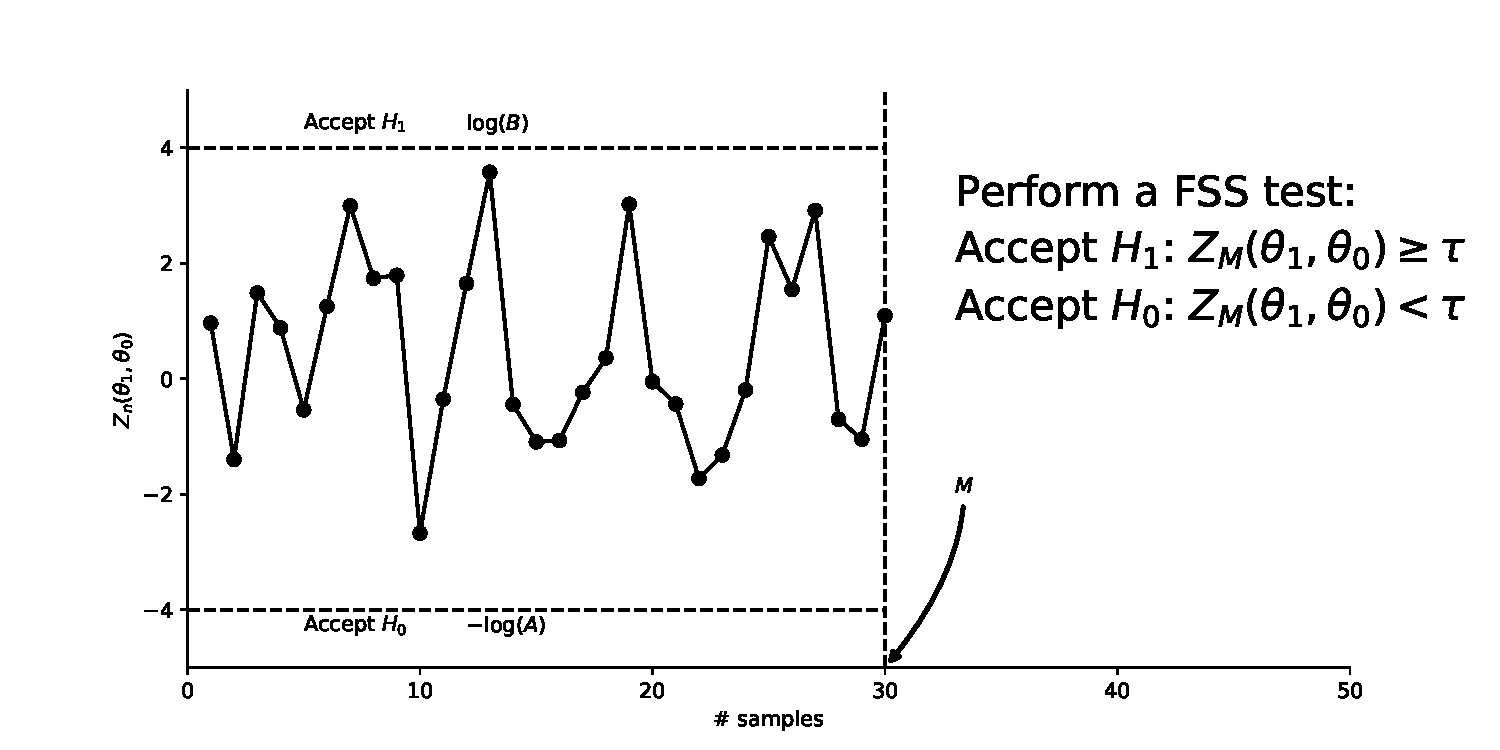
\includegraphics[width=0.8\textwidth]{images/truncated_sprt}
\caption{Example of the Truncated SPRT procedure.}
\label{fig:trunc_sprt}
\end{figure}

One chooses $A, B, M, \tau$ to control the error probabilities at the desired levels $\alpha$ and $\beta$. The key result that makes the experimental design possible is the following bound on the error probabilities derived in \citet{tantara1977}:
\begin{equation}\label{eq:design_bound}
\begin{split}
P_{\theta_0}(D = 1) &\leq \alpha_{SPRT} + \alpha_{FSS} \\
P_{\theta_1}(D = 0) &\leq \beta_{SPRT} + \beta_{FSS}.
\end{split}
\end{equation}
Note that this follows from a union bound between the SPRT and FSS parts of the test.

With the bound in Equation \ref{eq:design_bound}, we can describe how to choose the test's parameters. We begin by choosing mixing weights $c_1, c_2 \in \left[0, 1\right]$ such that
\begin{equation}
\begin{split}
\alpha_{FSS} = c_1 \alpha, \quad &\alpha_{SPRT} = (1 - c_1) \alpha \\
\beta_{FSS} = c_2 \beta, \quad &\beta_{SPRT} = (1 - c_2) \beta.
\end{split}
\end{equation}
We then use Wald's recommendations to set the thresholds of the SPRT:
\begin{equation}
\begin{split}
A &= \frac{1 - \alpha_{SPRT}}{\beta_{SPRT}} \\
B &= \frac{1 - \beta_{SPRT}}{\alpha_{SPRT}}. \\
\end{split}
\end{equation}
Assuming that we can approximate the CDF of $Z_n(\theta_1, \theta_0)$ with a normal (true for the exponential family), we set the truncation level $M$ and FSS threshold $\tau$ to control the FSS error probabilities:
\begin{equation}
\begin{split}
M &= \frac{1}{(\mu_{\theta_1} - \mu_{\theta_0})^2} \left(\sigma_{\theta_1} z_{\beta_{FSS}} + \sigma_{\theta_0}z_{\alpha_{FSS}}\right)^2 \\
\tau &= \frac{\sqrt{M}}{\mu_{\theta_1} - \mu_{\theta_0}} \left(\mu_{\theta_1} \sigma_{\theta_0} z_{\alpha_{FSS}} + \mu_{\theta_0} \sigma_{\theta_1} z_{\beta_{FSS}}\right)
\end{split}
\end{equation}
where $\mu_{\theta} = E_{\theta}\left[Z_1(\theta_1, \theta_0)\right]$ and $\sigma^2_{\theta} = \text{Var}_{\theta}\left[Z_1(\theta_1, \theta_0)\right]$. Because $\alpha_{FSS} + \alpha_{SPRT} = 1$ and $\beta_{FSS} + \beta_{SPRT} = 1$, these settings achieve the desired error control.

\subsection{Choosing the Mixing Weights}

Now that we know how to design the test the question remains how to choose the mixing weights $c_1$ and $c_2$. If the truncation level is unconstrained in the experimental design, it is recommended to monitor the following quantities:
\begin{equation}\label{eq:c_optim}
\frac{E_{\theta_{*}}[T\,]}{M_{FSS}}, \, \frac{M}{M_{FSS}}  \, \text{ and } \, \frac{E_{\theta_0}[T\,]}{E_{\theta_0}[T_{SPRT}]}, \frac{E_{\theta_1}[T\,]}{E_{\theta_1}[T_{SPRT}]}.
\end{equation}
Recall that we are designing a truncated test so that we take less samples than the FSS test on average. In addition, we would like to match the optimal performance of the SPRT at $\theta_0$ and $\theta_1$. Therefore, we would like the first two quantities to be smaller than one and the last two quantities to be close to one.

We consider two different experimental designs. The first is one in which the truncation level is allowed to be unconstrained and

%as well as how the test compares with other popular sequential tests. We answer these questions through numerical experimentation in the next section.

\section{Numerical Results}

For our simulations we will consider how the test performs when the data comes from a Gaussian distribution. In particular, consider $X \iidsim N(\theta, 1)$ and we want to test $H_0 : \theta \leq -\delta$ vs. $H_1 : \theta \geq \delta$. The FSS thresholds are
\begin{equation}
\begin{split}
M &= \frac{(z_{\alpha_{FSS}} + z_{\beta_{FSS}})^2}{4 \delta^2} \\
\tau &= \sqrt{M} \delta (z_{\alpha_{FSS}} - z_{\beta_{FSS}}).
\end{split}
\end{equation}

\begin{figure}
\centering
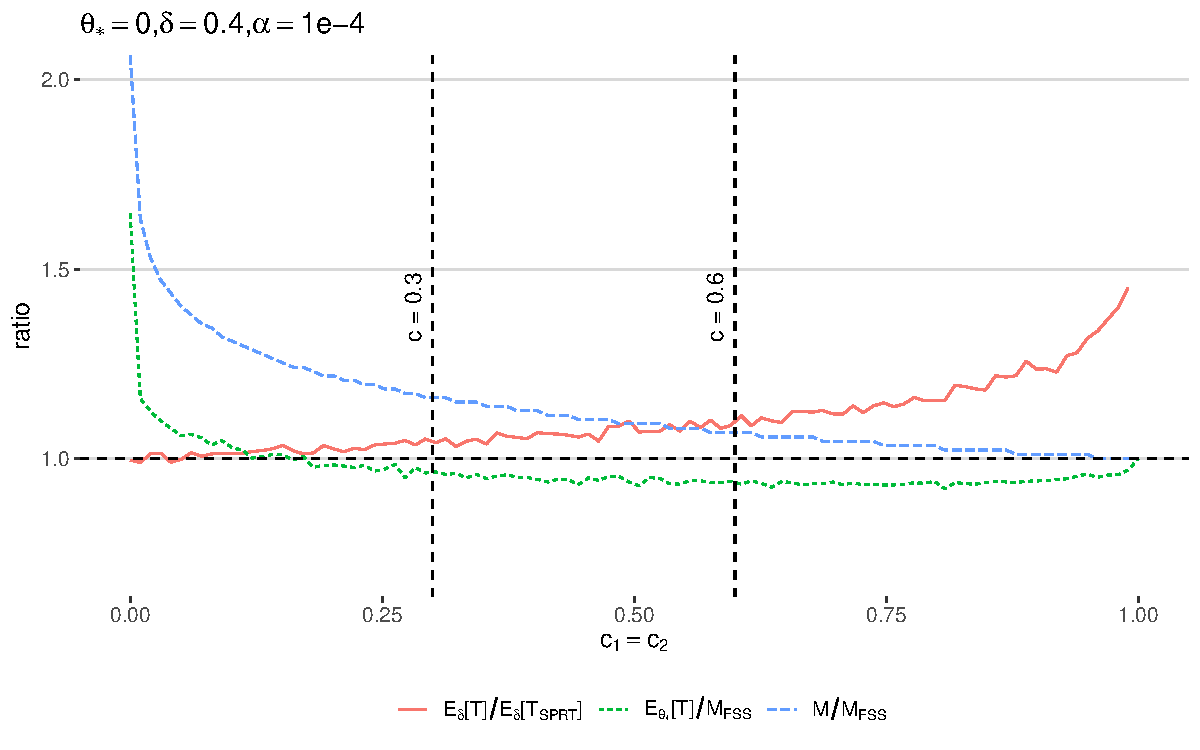
\includegraphics[width=0.8\textwidth]{images/c1_c2_ratios}
\caption{Effect of $c_1$ and $c_2$ on the quantities in Equation \ref{eq:c_optim} for the Gaussian example.}
\end{figure}

\subsection{Comparison with Other Sequential Tests}\label{sec:comparisons}

\begin{figure}
\centering
\begin{subfigure}{0.49\textwidth}
    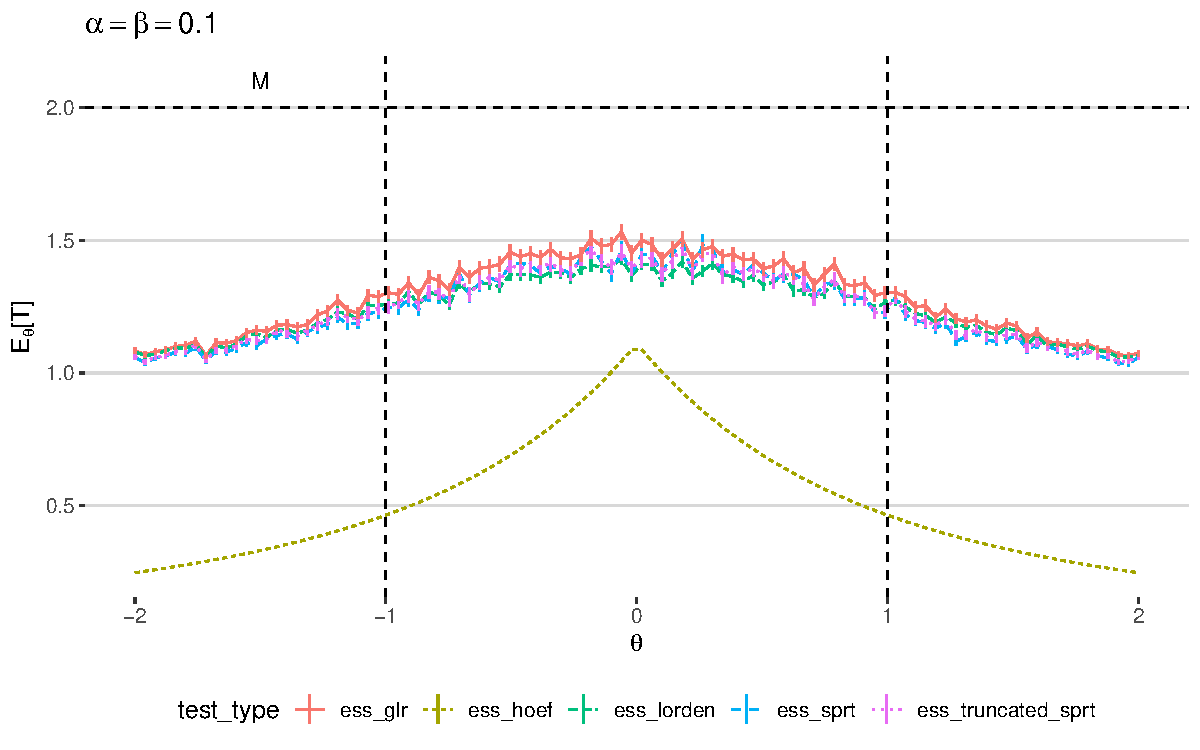
\includegraphics[width=\textwidth]{images/ess_alpha1e1}
\end{subfigure}
\hfill
\begin{subfigure}{0.49\textwidth}
    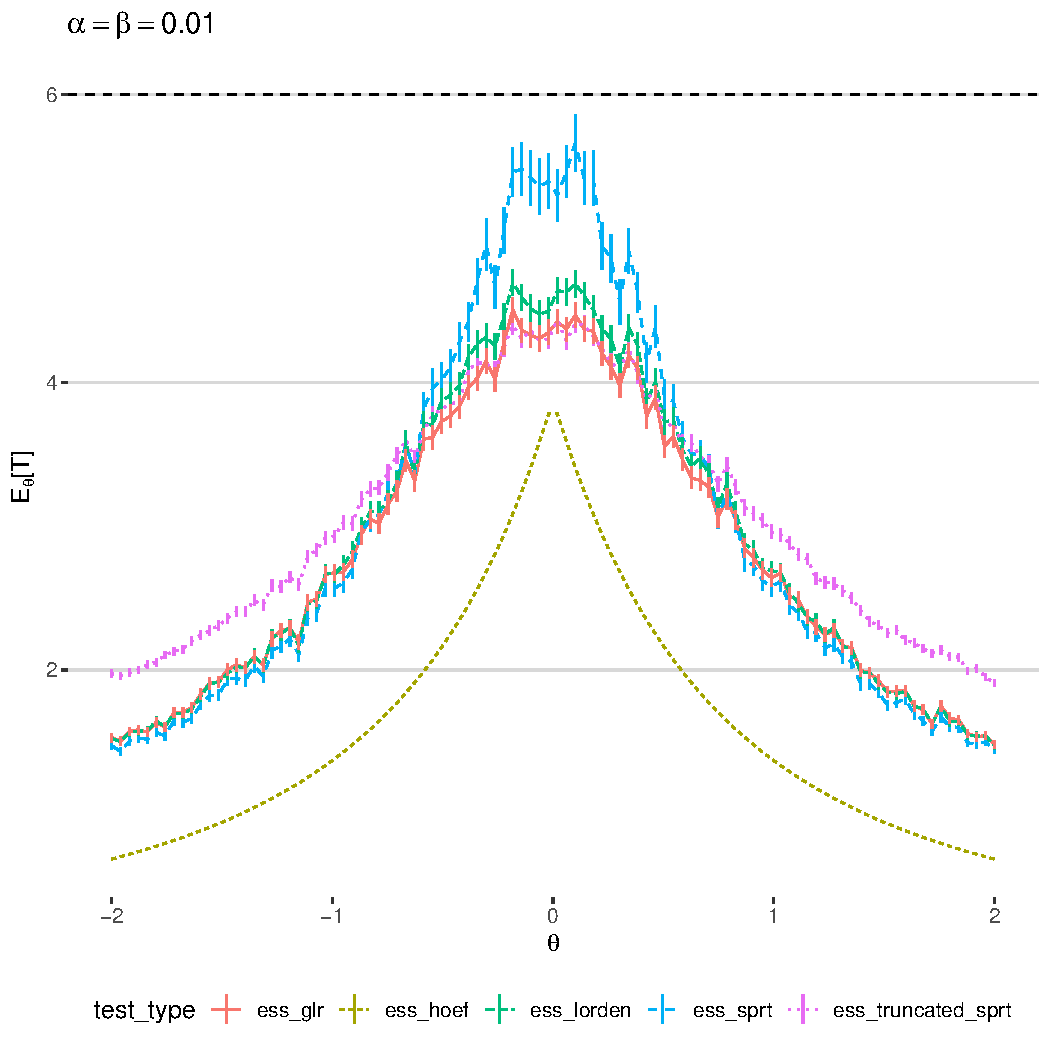
\includegraphics[width=\textwidth]{images/ess_alpha1e2}
\end{subfigure}
\begin{subfigure}{0.49\textwidth}
    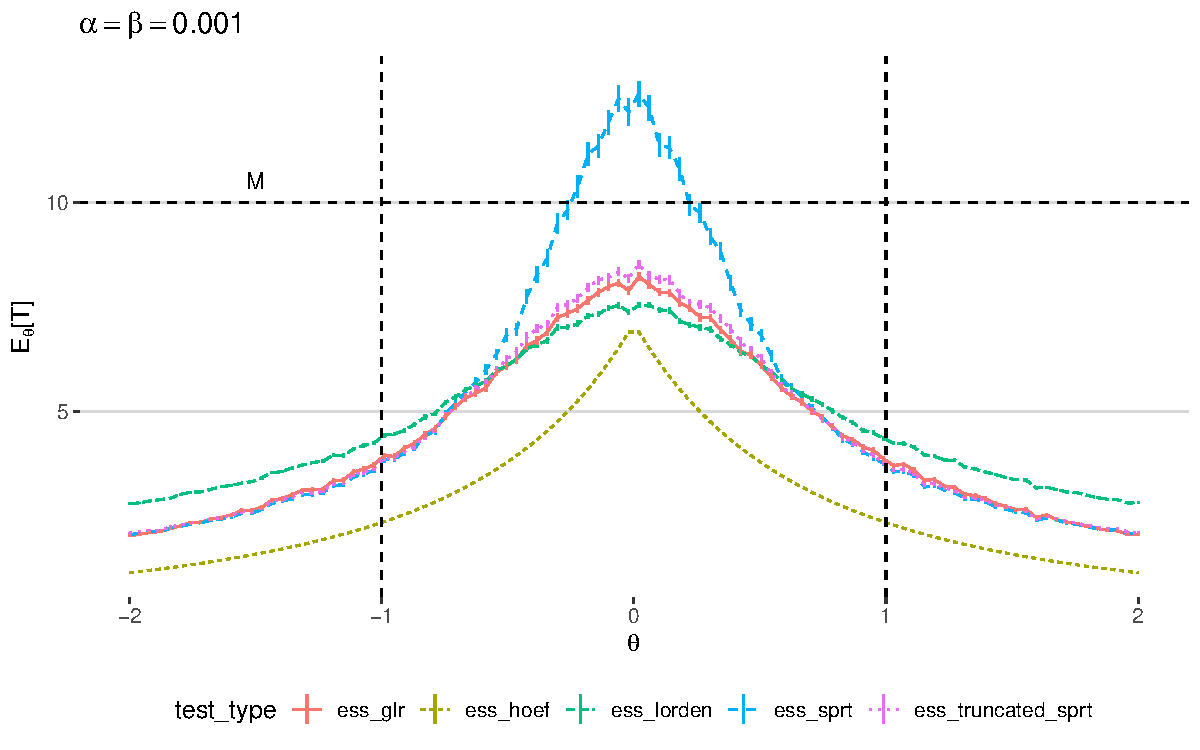
\includegraphics[width=\textwidth]{images/ess_alpha1e3}
\end{subfigure}
\hfill
\begin{subfigure}{0.49\textwidth}
    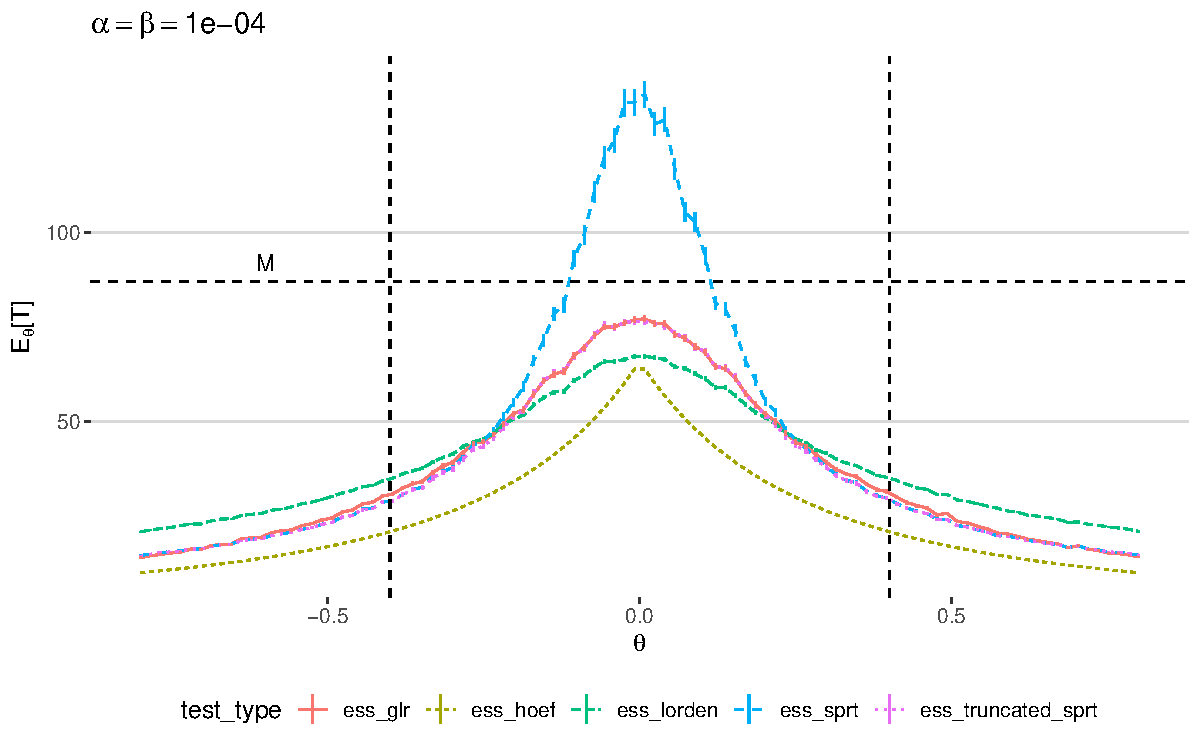
\includegraphics[width=\textwidth]{images/ess_alpha1e4}
\end{subfigure}

\caption{Comparison for the SPRT, Truncated SPRT, Lorden's 2-SPRT, and the GLR test when $X_i \iidsim N(\theta, 1)$, $\theta_0 = -\theta_1 = 1$, and thresholds are choosen such that the error probabilities are $\alpha = \beta = 0.1, 10^{-2}, 10^{-3}, 10^{-4}$. The mixing proportion was set to $c_1 = c_2 = 0.5$ for the Truncated SPRT. For large error probabilities (0.1 or $10^{-2}$, the Truncated SPRT generally performs worse or equivalent to Lorden's 2-SPRT and the GLR test. For small error probabilities, the Truncated SPRT has uniformly lower ESS between 0.5 and $-0.5$, but has much heavy tails for large $\theta$. All tests besides the SPRT have a smaller sample size on average than the equivalent FSS test.}
\end{figure}

\section{Conclusion}

\newpage
\bibliographystyle{asa}
\bibliography{reference}

\end{document}
